\documentclass[a4paper,11pt,twoside]{article}

\usepackage{amsmath}
\usepackage{amssymb}
\usepackage[english]{babel}
\usepackage{cite}
\usepackage{color}
\usepackage{hyperref}
\usepackage{graphicx}
\usepackage{amsthm}
\usepackage{xspace}

\title{Assignment 3 -- literature overview}
\author{\href{mailto:pkok@science.uva.nl}{Patrick de Kok}}

% markup for geometric terminology
\newcommand{\textgt}[1]{\textsf{#1}\xspace} 
% geometric terminology
\newcommand{\pBrush}{\textgt{Brush}}
\newcommand{\pBrushes}{\textgt{Brushes}}
\newcommand{\ebrush}{\textgt{brush}}
\newcommand{\ebrushes}{\textgt{brushes}}
\newcommand{\pLine}{\textgt{Line}}
\newcommand{\pLines}{\textgt{Lines}}
\newcommand{\eline}{\textgt{line}}
\newcommand{\elines}{\textgt{lines}}
\newcommand{\pPencil}{\textgt{Pencil}}
\newcommand{\pPencils}{\textgt{Pencils}}
\newcommand{\epencil}{\textgt{pencil}}
\newcommand{\epencils}{\textgt{pencils}}

\newcommand{\pPlane}{\textgt{Plane}}
\newcommand{\pPlanes}{\textgt{Planes}}
\newcommand{\eplane}{\textgt{plane}}
\newcommand{\eplanes}{\textgt{planes}}
\newcommand{\pPoint}{\textgt{Point}}
\newcommand{\pPoints}{\textgt{Points}}
\newcommand{\epoint}{\textgt{point}}
\newcommand{\epoints}{\textgt{points}}
\newcommand{\pRegulus}{\textgt{Regulus}}
\newcommand{\pReguli}{\textgt{Reguli}}
\newcommand{\pRegPen}{\textgt{Regulus Pencil}}
\newcommand{\pRegPens}{\textgt{Regulus Pencils}}

% Math type specifying fonts
\newcommand{\V}[1]{\ensuremath{\mathbf{#1}}}

% Math-like symbols
\newcommand{\reals}{\ensuremath{\mathbb{R}}}
\newcommand{\RL}{\ensuremath{\reals^{3,3}}}
\newcommand{\en}{\ensuremath{\mathbin{\mbox{and}}}}
\newcommand{\of}{\ensuremath{\mathbin{\mbox{or}}}}
\newcommand{\eql}{\ensuremath{\Leftrightarrow}}

\newtheorem{theorem}{Theorem}
\newtheorem{question}{Question}
\newtheorem{lemma}{Lemma}

\definecolor{nicered}{rgb}{0.6, 0, 0.24}
\definecolor{nicegreen}{rgb}{0.0, 0.5, 0.24}
\definecolor{niceblue}{rgb}{0, 0.4, 1}

\hypersetup{
  colorlinks=true,
  urlcolor=nicegreen,
  linkcolor=niceblue,
  citecolor=nicered,
}

\begin{document}
\maketitle
\begin{abstract}
For this thesis, I will develop an extension of GAViewer, a visualizing calculator for conformal geometric algebra.  The extension will implement a model of projective geometry that is based on Pl\"ucker coordinates.
\end{abstract}

Just as linear algebra, geometric algebra is an algebra over a given vector space $\reals^n$.  The difference lies in its operations; whereas linear algebra relies on matrix manipulations which cannot always be inverted, geometric algebra's base operation is the geometric product.  From this inversible product, one can deduce the inner product, known from linear algebra, and the outer product.  The outer product grants the user access to the exterior algebra $\bigwedge \reals^n$.  The outer product of $\V{A}, \V{B} \in \bigwedge \reals^n: \V{A} \wedge \V{B}$ represents the set of elements that are linear combinations of its operands $\left\{\alpha \V{A} + \beta \V{B} \mid \alpha, \beta \in \reals \right\}$

There are already several models of geometry in use in the geometric algebra community, of which the conformal model is the most popular and widely known~\cite{TheBook}.  Although usable in many cases, the transformations of the conformal model are a subset of those of the projective model. The projective transformations are an important class of operations within computer vision and computer graphics. 

GAViewer is a visualization and computing tool for the 3-dimensional Euclidean and conformal models of geometric algebra, developed by Daniel Fontijne at the University of Amsterdam~\cite{GAViewer}.  It allows the user to do calculations in geometric algebra, and shows the results, both numerical as well as graphical.  Moreover, it allows the user to rotate, translate and zoom the viewport, as well as to manipulate the displayed elements.  The variables in which they are stored are automatically updated, and, if desired by the user, other objects that are parameterized by the manipulated object, may be updated dynamically as well.

Recently, Li and Zhang~\cite{Hongbo} have found a way to model projective geometry, using a 6 dimensional representation space $\RL$ with a special metric, which allows three basis vectors to square to $-1$.  Using Pl\"ucker coordinates~\cite{Hongbo,Pottmann2}, lines in 3-dimensional Euclidean space $\mathbb{E}^3$ are represented in the representation space by vectors $\V{v}^2 = \V{v} \V{v} = \V{v} \cdot \V{v} = 0$.  As a consequence, there also exist vectors in the representation space $\V{w}^2 \not= 0$ which do not represent lines in $\mathbb{E}^3$.  Different geometrical objects are generated by the outer product over lines and non-lines.  For example, for two intersecting lines $\ell_1, \ell_2$, the outer product $\ell_1 \wedge \ell_2$ represents a pencil, the collection of all lines that are in the same plane as $\ell_1$ and $\ell_2$, and pass through the same point.  Taking the outer product of this pencil with a third intersecting line that does not lie in the same plane, results in a bundle; the set of all lines intersecting in a certain point.  This could be used to represent points in our space of lines.

In their article, Li and Zhang have not discussed what each element in their algebra might represent.  Barrau~\cite{Barrau1,Barrau2} and Pottmann and Wallner~\cite{Pottmann2,Pottmann3} have investigated the objects that can be represented in a 6-dimensional space with Pl\"ucker coordinates, both using a different algebra from ours.  Pottmann and Wallner use linear algebra, while Barrau's algebra has less expressive power.  

In the first part of this thesis, the elements of $\RL$ are described.  Assuming that the representation spaces of Barrau and Pottmann and Wallner are the same as that of this study, a translation will be presented.

In the second part, an extension of GAViewer will be represented that will enable the user to work with, and visualize $\RL$.  Although the operations of conformal geometry are a subset of projective geometry, it does not mean the geometric objects of the conformal model are a subset of the projective model.  The conformal model uses the sphere with radius $0$ as its base element, and infinity should be treated specially (in fact, it is represented as a separate dimension).  The base element of our projective model is a line.  Also, due to the homogeneous nature of Pl\"ucker coordinates, infinity can be treated as any other number.  Therefore, one cannot assume it trivial to represent the items of the projective model in the conformal model.  Another non-triviality is the user interaction with the elements.  Even though only differentiable transformations will be considered for user interaction, only rotation and translation are implemented by default.  Other transformations might not be as intuitive to interact with for the user.  For this kind of interaction to work smoothly, it would be preferable that transformations in $\mathbb{E}^3$ correspond to a similar action in $\RL$.

\begin{figure}[t]
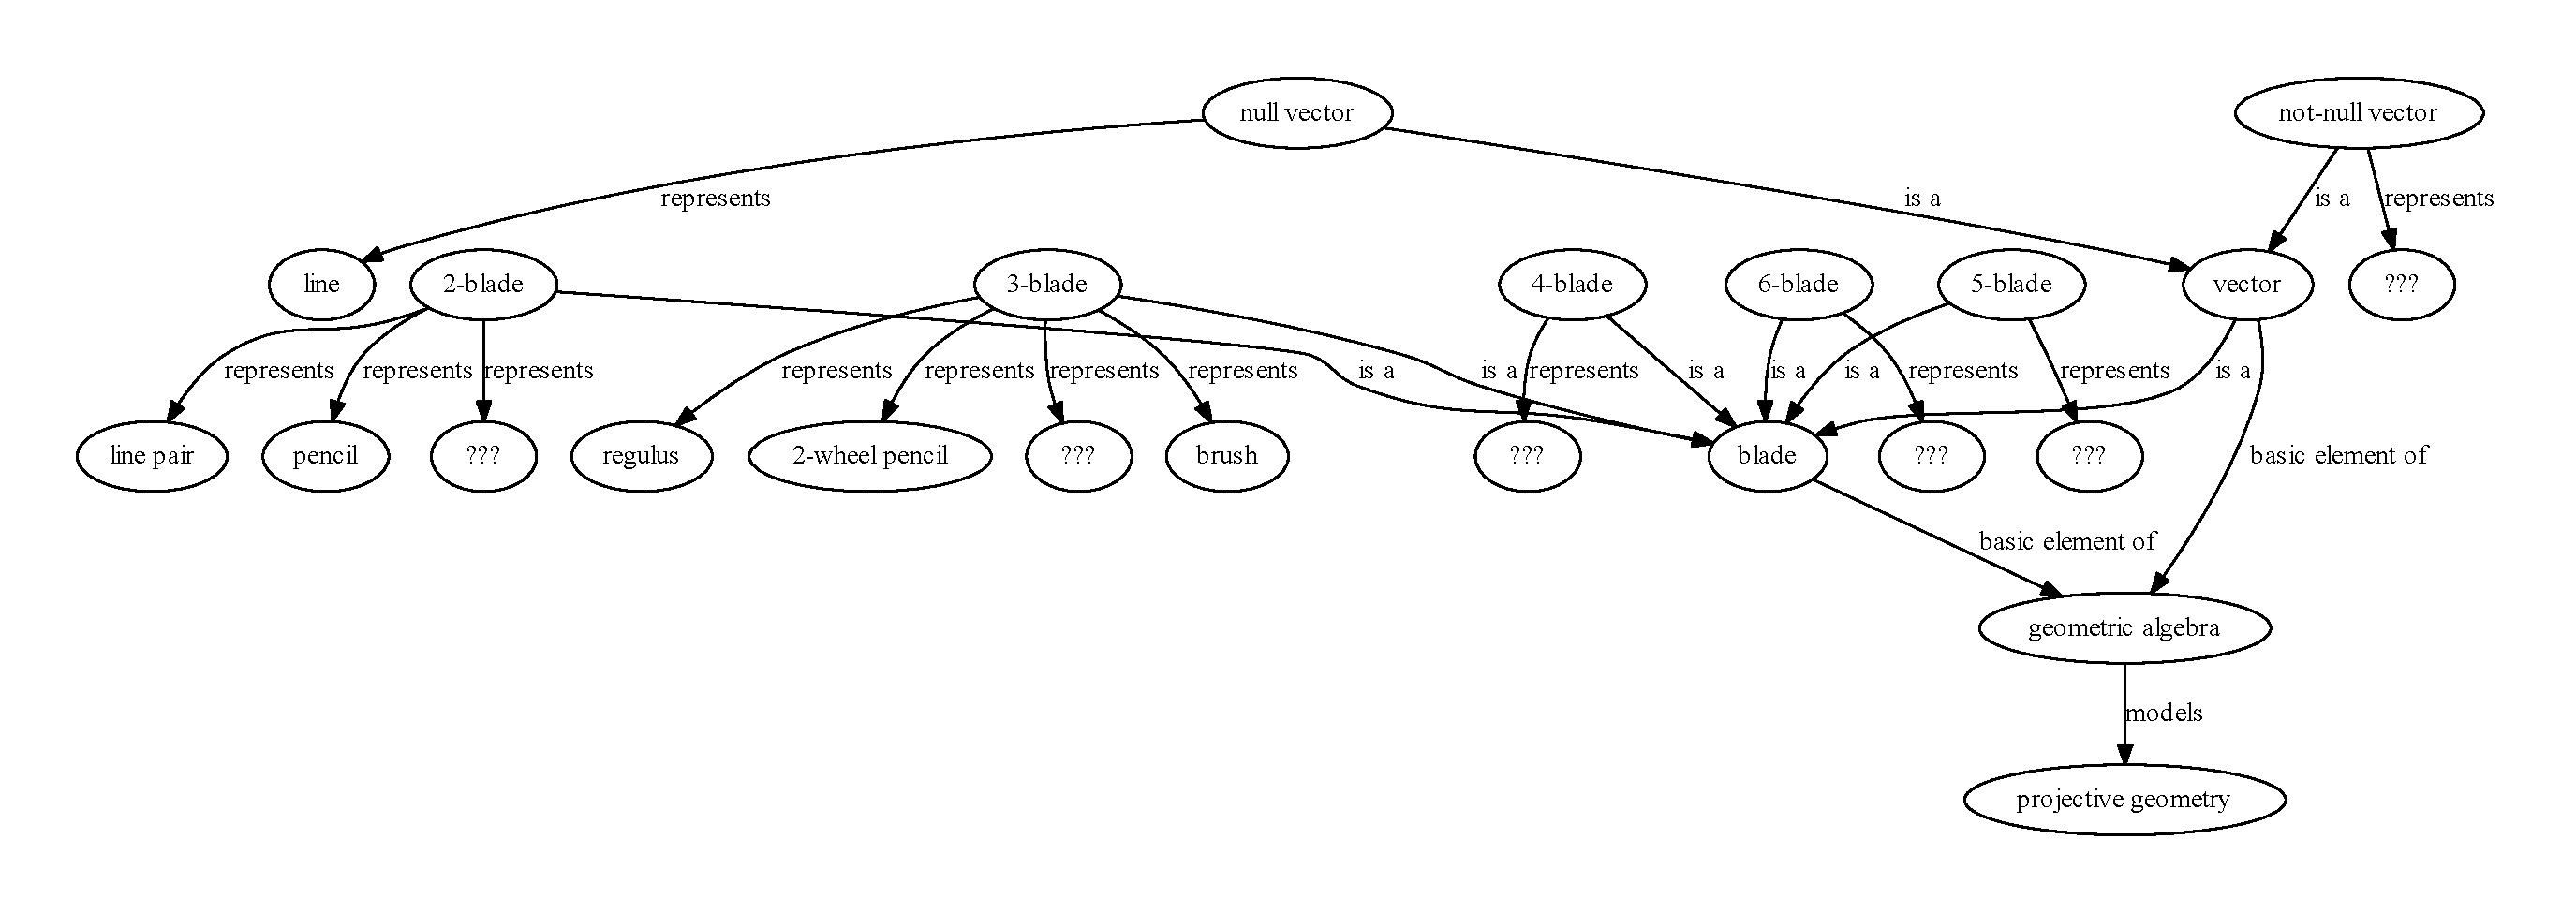
\includegraphics[width=1.0\textwidth]{conceptmap.pdf}
\caption{Concept map, as requested.}
\end{figure}

\bibliography{citations}{}
\bibliographystyle{plain}
\end{document}
